\documentclass[border=6pt]{standalone}
\usepackage{tikz}
\usetikzlibrary{arrows.meta,positioning}
\begin{document}
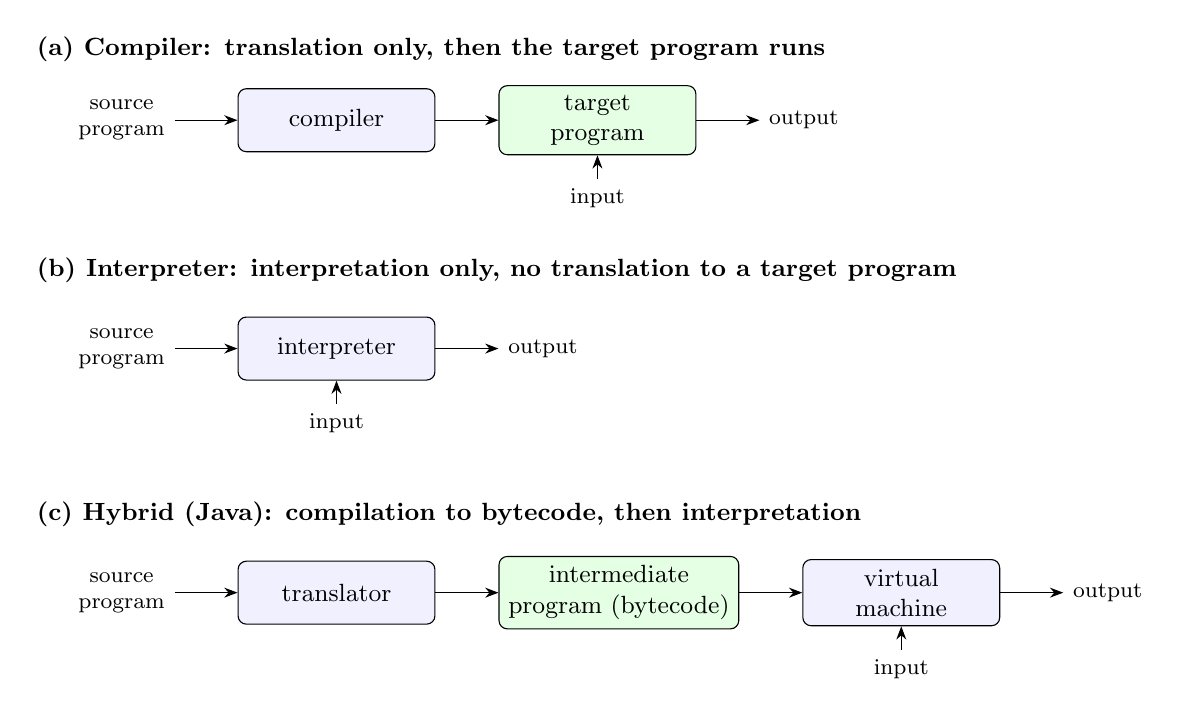
\begin{tikzpicture}[>=Stealth,font=\small,node distance=0.8cm,
 blk/.style={draw,rounded corners=3pt,minimum width=2.5cm,minimum height=0.8cm,align=center,fill=blue!6},
 io/.style={align=center,font=\footnotesize},
 hd/.style={font=\small\bfseries,anchor=west}]
% compiler
\node[hd] at (-1.2,0.9) {(a) Compiler: translation only, then the target program runs};
\node[io] (a1) at (0,0) {source\\program};
\node[blk,right=of a1] (a2) {compiler};
\node[blk,right=of a2,fill=green!10] (a3) {target\\program};
\node[io,right=of a3] (a4) {output};
\node[io,below=0.3cm of a3] (ain) {input};
\draw[->] (a1)--(a2); \draw[->] (a2)--(a3); \draw[->] (a3)--(a4); \draw[->] (ain)--(a3);
% interpreter
\node[hd] at (-1.2,-1.9) {(b) Interpreter: interpretation only, no translation to a target program};
\node[io] (b1) at (0,-2.9) {source\\program};
\node[blk,right=of b1] (b2) {interpreter};
\node[io,right=of b2] (b3) {output};
\node[io,below=0.3cm of b2] (bin) {input};
\draw[->] (b1)--(b2); \draw[->] (b2)--(b3); \draw[->] (bin)--(b2);
% hybrid
\node[hd] at (-1.2,-5.0) {(c) Hybrid (Java): compilation to bytecode, then interpretation};
\node[io] (c1) at (0,-6.0) {source\\program};
\node[blk,right=of c1] (c2) {translator};
\node[blk,right=of c2,fill=green!10] (c3) {intermediate\\program (bytecode)};
\node[blk,right=of c3] (c4) {virtual\\machine};
\node[io,right=of c4] (c5) {output};
\node[io,below=0.3cm of c4] (cin) {input};
\draw[->] (c1)--(c2); \draw[->] (c2)--(c3); \draw[->] (c3)--(c4); \draw[->] (c4)--(c5); \draw[->] (cin)--(c4);
\end{tikzpicture}
\end{document}
